\documentclass[7Sketches]{subfiles}
\begin{document}

%------------ Chapter ------------%
\chapter*{Preface}

Category theory is becoming a central hub for all of pure mathematics.\index{category theory!as central hub of mathematics} It is unmatched in its ability to organize and layer abstractions, to find commonalities between structures of all sorts, and to facilitate communication between different mathematical communities.

But it has also been branching out into science, informatics, and industry. We believe that it has the potential to be a major cohesive force in the world, building rigorous bridges between disparate worlds, both theoretical and practical. The motto at MIT is \emph{mens et manus}, Latin for mind and hand. We believe that category theory---and pure math in general---has stayed in the realm of mind for too long; it is ripe to be brought to hand.

%-------- Section --------%
\section*{Purpose and audience}

The purpose of this book is to offer a self-contained tour of applied category theory. It is an invitation to discover advanced topics in category theory through concrete real-world examples. Rather than try to give a comprehensive treatment of these topics---which include adjoint functors, enriched categories, proarrow equipments, toposes, and much more---we merely provide a taste of each. We want to give readers some insight into how it feels to work with these structures as well as some ideas about how they might show up in practice.

The audience for this book is quite diverse: anyone who finds the above description intriguing. This could include a motivated high school student who hasn't seen calculus yet but has loved reading a weird book on mathematical logic they found at the library. Or a machine-learning researcher who wants to understand what vector spaces, design theory, and dynamical systems could possibly have in common. Or a pure mathematician who wants to imagine what sorts of applications their work might have. Or a recently-retired programmer who's always had an eerie feeling that category theory is what they've been looking for to tie it all together, but who's found the usual books on the subject impenetrable.

For example, we find it something of a travesty that in 2018 there is almost no introductory material available on monoidal categories. Even beautiful modern introductions to category theory, e.g.\ by Riehl or Leinster, do not include anything on this rather central topic. The only exceptions we can think of are \cite[Chapter 3]{Coecke.Kissinger:2017a} and \cite{coecke2010categories}, each of which has a very user-friendly introduction to monoidal categories; however, readers who are not drawn to physics may not think to look there.\index{category theory!books on}

The basic idea of monoidal categories is certainly not too abstract; modern human intuition seems to include a pre-theoretical understanding of monoidal categories that is just waiting to be formalized. Is there anyone who wouldn't correctly understand the basic idea being communicated in the following diagram?\index{monoidal category}\index{wiring diagram}\index{cooking}
\[
\begin{tikzpicture}[oriented WD, align=center, bbx=1.2cm, bby=2ex]
	\node[bb={4}{1}, bb min width=.9in] (filling) {make\\lemon\\filling};
	\node[bb={2}{1}, bb min width=.9in, below=of filling] (meringue) {make\\meringue};
	\node at ($(filling.west)!.5!(meringue.west)$) (helper) {};
	\node[bb={1}{2}, left = of helper] (separate) {separate\\egg};
	\node[bb={2}{1}, above right = -2 and 1 of filling] (fill) {fill crust};
	\node[bb={2}{1}, below right = of fill] (finish) {add\\meringue};
	\node[bb={0}{0}, bb name=prepare lemon meringue pie, fit={(separate) (meringue) ($(fill.north)+(0,2)$) (finish)}] (pie) {};
%
\begin{scope}[font=\tiny]
	\draw (pie.west|-fill_in1) to node[pos=.25, above] {prepared crust} (fill_in1);
	\draw (pie.west|-filling_in1) to node[above] {lemon} (filling_in1);
	\draw (pie.west|-filling_in2) to node[above] {butter} (filling_in2);
	\draw (pie.west|-filling_in3) to node[above] {sugar} (filling_in3);
	\draw (pie.west|-separate_in1) to node[above] {egg} (separate_in1);
	\draw (pie.west|-meringue_in2) to node[above] {sugar} (meringue_in2);
	\draw (separate_out1) to node[above] {yolk} (filling_in4);
	\draw (separate_out2) to node[fill=white, inner sep=0.8pt] {white} (meringue_in1);
	\draw (filling_out1) to node[fill=white, inner sep=0.8pt] {lemon\\filling} (fill_in2);
	\draw (fill_out1) to node[fill=white, inner sep=0.8pt] {unbaked\\lemon pie} (finish_in1);
	\draw let \p1=(fill.east|-meringue_out1), \n1=\bbportlen in
		(meringue_out1) to node[above] {meringue} (\x1+\n1,\y1) to (finish_in2);
	\draw (finish_out1) to node[above] {unbaked\\pie} (finish_out1-|pie.east);
\end{scope}
\end{tikzpicture}
\]
Many applied category theory topics seem to take monoidal categories as their jumping-off point. So one aim of this book is to provide a reference---even if unconventional---for this important topic.

We hope this book inspires both new visions and new questions. We intend it
to be self-contained in the sense that it is approachable with minimal
prerequisites, but not in the sense that the complete story is told here. On the
contrary, we hope that readers use this as an invitation to further reading, to
orient themselves in what is becoming a large literature, and to discover new applications for themselves.

This book is, unashamedly, our take on the subject. While the abstract
structures we explore are important to any category theorist, the specific
topics have simply been chosen to our personal taste. Our examples are ones that
we find simple but powerful, concrete but representative, entertaining but in a
way that feels important and expansive at the same time. We hope our readers
will enjoy themselves and learn a lot in the process.

%-------- Section --------%
\section*{How to read this book}

The basic idea of category theory---which threads through every chapter---is that if one pays careful attention to structures and coherence, the resulting systems will be extremely reliable and interoperable. For example, a category involves several structures: a collection of objects, a collection of morphisms relating objects, and a formula for combining any chain of morphisms into a morphism. But these structures need to \emph{cohere} or work together in a simple commonsense way: a chain of chains is itself a long chain, so combining a chain of chains should be the same as combining the long chain. That's it!\index{morphism}

We will see structures and coherence come up in pretty much every definition we
give: ``here are some things and here are how they fit together.'' We ask the
reader to be on the lookout for structures and coherence as they read the book,
and to realize that as we layer abstraction upon abstraction, it is the coherence
that makes all the parts work together harmoniously in concert.\index{coherence}

Each chapter in this book is motivated by a real-world topic, such as electrical circuits, control theory, cascade failures, information integration, and hybrid systems. These motivations lead us into and through various sorts of category-theoretic concepts. We generally have one motivating idea and one category-theoretic purpose per chapter, and this forms the title of the chapter, e.g.\ Chapter 4 is ``Collaborative design: profunctors, categorification, and monoidal categories.''

In many math books, the difficulty is roughly a monotonically-increasing function of the page number. In this book, this occurs in each chapter, but not so much in the book as a whole. The chapters start out fairly easy and progress in difficulty.
\[
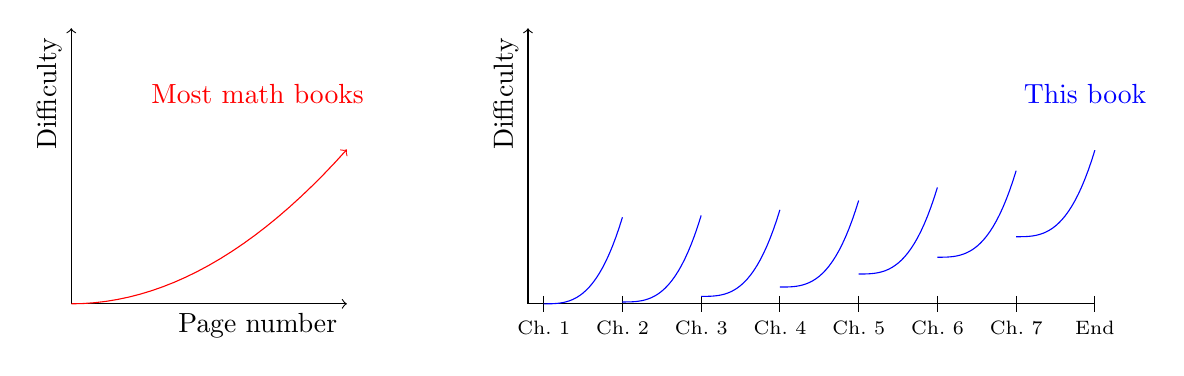
\begin{tikzpicture}
  \draw[->] (0,0) -- (3.5,0) node[below left] (p) {Page number};
  \draw[->] (0,0) -- (0,3.5) node[above left, rotate=90] (d) {Difficulty};
  \draw[color=red, domain=0:3.5, ->] plot (\x,{.16*\x^2)});
  \node[red] at (p|-d) {Most math books};
%
  \draw (5.8,0) -- (13,0) node[below left] (p) {};
  \draw[->] (5.8,0) -- (5.8,3.5) node[above left, rotate=90] (d) {Difficulty};
  \foreach \i in {1,...,7} {
  	\draw (\i+5,.1) to (\i+5,-.1) node[below, font=\scriptsize] {Ch.\ \i};
    \draw[color=blue, domain=\i+5:\i+6] plot (\x,{1.1*(\x-\i-5)^3+((\i-1)/6.5)^2});
	}
 	\draw (13,.1) to (13,-.1) node[below, font=\scriptsize] {End};
  \node[blue] at (p|-d) {This book};
\end{tikzpicture}
\]
The upshot is that if you find the end of a chapter very difficult, hope is certainly not lost: you can start on the next one and make good progress. This format lends itself to giving you a first taste now, but also leaving open the opportunity for you to come back to the book at a later date and get more deeply into it. But by all means, if you have the gumption to work through each chapter to its end, we very much encourage that!

We include about 240 exercises throughout the text, with solutions in \cref{chap.solutions}. Usually these exercises are fairly straightforward; the only thing they demand is that the reader changes their mental state from passive to active, rereads the previous paragraphs with intent, and puts the pieces together. A reader becomes a \emph{student} when they work the exercises; until then they are more of a tourist, riding on a bus and listening off and on to the tour guide. Hey, there's nothing wrong with that, but we do encourage you to get off the bus and make direct contact with the native population and local architecture as often as you can.

%-------- Section --------%
\section*{Acknowledgments}

Thanks to Jared Briskman, James Brock, Ronnie Brown, Thrina Burana, David Chudzicki, Jonathan
Castello, Margo Crawford, Fred Eisele, David Ellerman, Cam Fulton, Bruno
Gavranovi\'c, Sebastian Galkin, John Garvin, Peter Gates, Juan Manuel Gimeno,
Alfredo G\'omez, Leo Gorodinski, Jason Grossman, Jason Hooper, Yuxi Liu, Jes\'us
L\'opez, MTM, Nicol\`o Martini, Martin MacKerel, Pete Morcos, Nelson Niu, James
Nolan, Dan Oneata, Paolo Perrone, Thomas Read, Rif A.  Saurous, Dan Schmidt,
Samantha Seaman, Marcello Seri, Robert Smart, Valter Sorana, Adam
Theriault-Shay, Emmy Trewartha, Sergey Tselovalnikov, Andrew Turner, Joan
Vazquez, Daniel Wang, Jerry Wedekind for helpful comments and conversations.

We also thank our sponsors at the AFOSR; this work was supported by grants
FA9550--14--1--0031 and FA9550--17--1--0058.

Finally, we extend a very special thanks to John Baez for running an
\href{https://forum.azimuthproject.org/categories/applied-category-theory-course}{online
course} on this material and generating tons of great feedback.


%-------- Section --------%
\section*{Personal note}

Our motivations to apply category theory outside of math are, perhaps naively,
grounded in the hope it can help bring humanity together to solve our big
problems. But category theory is a tool for thinking, and like any tool it can
be used for purposes we align with and those we don't. 

In this personal note, we ask that readers try to use what they learn in this
book to do something they would call ``good,'' in terms of contributing to the
society they'd want to live in. For example, if you're planning to study this
material with others, consider specifically inviting someone from an
under-represented minority---a group that is more highly represented in society
than in upper-level math classes---to your study group. As another example,
perhaps you can use the material in this book to design software that helps
people relate to and align with each other. What's the mathematics of a
well-functioning society?

The way we use our tools affects all our lives. Our society has seen the
results---both the wonders and the waste---resulting from rampant selfishness.
We would be honored if readers found ways to use category theory as part of an
effort to connect people, to create common ground, to explore the cross-cutting
categories in which life, society, and environment can be represented, and to end the
ignorance entailed by limiting ourselves to a singular ontological perspective
on anything.

If you do something of the sort, please let us and the community know about it.
\vspace{1cm}


\flushright
Brendan Fong and David I.\ Spivak

Cambridge MA, October 2018


%\begin{adjustwidth}{.6\textwidth}{0pt}
%\noindent \textit{Brendan Fong}\qquad \textit{David I.\ Spivak}
%
%\noindent Cambridge, MA.\quad  2018
%\end{adjustwidth}

\end{document}
